\documentclass[11pt]{homework}

\usepackage[UTF8]{ctex}
\usepackage{graphicx}
\usepackage{float} 
\usepackage{subfigure}
\usepackage{listings}
\lstset{breaklines=true}

\newcommand{\hwname}{封钰震}
\newcommand{\hwemail}{1951362}
\newcommand{\hwtype}{作业}
\newcommand{\hwnum}{2-Java基础}
\newcommand{\hwclass}{Java语言程序设计}
\newcommand{\hwlecture}{}
\newcommand{\hwsection}{}

\usepackage{lipsum}

\begin{document}
\maketitle

\question*{编程环境}

  \subsection*{硬件环境}
  \begin{enumerate}
    \item 型号名称:MacBook Pro
    \item 处理器名称:Dual-Core Intel Core i5
    \item 内存:8 GB
  \end{enumerate}

  \subsection*{软件环境}

  系统版本:macOS 10.15.7

  \subsection*{运行环境}

  \begin{enumerate}
    \item JDK 14.0.2
  \end{enumerate}

\question*{设计思想}

\subsection*{走台阶——动态规划}
采用动态规划算法。对于第$n$个台阶而言,可以从第$n - 1$个台阶处跨一个台阶到达,也可以从第$n - 2$个台阶处跨两个台阶得到。因此,有:
\begin{gather*}
  f(n) = \begin{cases}
    1, n = 1\\
    2, n = 2\\
    f(n - 1) + f(n - 2)
  \end{cases}
\end{gather*}

其余问题不需要使用特别的算法,详见“执行过程”一节。

\question*{执行过程}

\subsection*{第一问}

首先,编写计算走台阶方法数的\verb|walkOnStep|函数。
\lstset{language=java}
  \begin{lstlisting}
    public class Main {
      private static int walkOnStep(int numOfStep) {
        int n1 = 1, n2 = 2, temp = n2;
        // f(n) = f(n - 1) + f(n - 2)
        if (numOfStep == 1) {
            return 1;
        }
        else if (numOfStep == 2) {
            return 2;
        }
        else {
            for (int i = 3; i <= numOfStep; i = i + 1) {
                temp = n2;
                n2 = n2 + n1;
                n1 = temp;
                // System.out.println(i + ": " + n2);
            }
            return n2;
        }
      }
    }
  \end{lstlisting}

再在\verb|main|函数中调用\verb|walkOnStep|函数并输出。
\lstset{language=java}
  \begin{lstlisting}
    public static void main(String[] args) {
        int num = Main.walkOnStep(24);
        System.out.println(num);
    }
  \end{lstlisting}

得到结果$f(24) = 75025$,程序输出如图\ref{q1_output}所示。

\begin{figure}
  \centering
  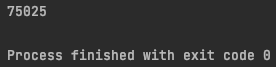
\includegraphics[width=0.5\textwidth]{q1_output}
  \caption{输出结果}
  \label{q1_output}
\end{figure}

\subsection*{第二问}
首先,在\verb|walkOnStep|函数添加输出:
\lstset{language=java}
  \begin{lstlisting}
    System.out.println(i + ": " + n2);
  \end{lstlisting}
(即前一问所示代码中被注释掉的一行)。

再在\verb|main|函数中调用\verb|walkOnStep|函数,给以较大的参数,如:
\lstset{language=java}
  \begin{lstlisting}
    int num = Main.walkOnStep(80);
  \end{lstlisting}

最后,得到输出结果,如图\ref{q2_output}所示。
\begin{figure}
  \centering
  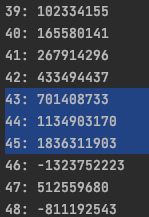
\includegraphics[width=0.3\textwidth]{q2_output}
  \caption{输出结果}
  \label{q2_output}
\end{figure}
因此,\verb|int|数据类型可以处理的台阶数的最大值为45。

\subsection*{第三问}
针对该问,在前两问程序的基础上增加了输入。用户可以选择运行该程序后输入台阶数(对应代码中\verb|if|分支),也可以选择在使用命令行运行该程序时输入台阶数(对应代码中\verb|else|分支)。修改后的\verb|main|函数如下:
\lstset{language=java}
  \begin{lstlisting}
    public static void main(String[] args) {
        int n = 1;
        try {
            if (args.length == 0) {
                System.out.print("Please input the number of steps: ");
                Scanner in = new Scanner(System.in);
                n = in.nextInt();
            }
            else {
                n = Integer.parseInt(args[0]);
            }
        } catch (Exception e) {
            e.printStackTrace();
            return;
        }

        int num = Main.walkOnStep(n);
        System.out.println(num);
    }
  \end{lstlisting}

下面使用命令行运行编译完成的\verb|.class|文件。

首先,找到\verb|Main.class|文件所在目录,如图\ref{q3_output_1}所示。
\begin{figure}
  \centering
  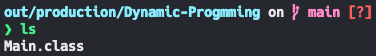
\includegraphics[width=0.5\textwidth]{q3_output_1}
  \caption{输出结果}
  \label{q3_output_1}
\end{figure}

使用\verb|java|程序启动Java虚拟机,虚拟机执行\verb|Main.class|文件中的字节码,未输入和输入参数的情形分别如图\ref{q3_output_2}和图\ref{q3_output_3}所示。
\begin{figure}
  \centering
  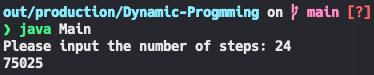
\includegraphics[width=0.5\textwidth]{q3_output_2}
  \caption{输出结果}
  \label{q3_output_2}
\end{figure}
\begin{figure}
  \centering
  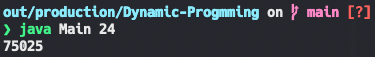
\includegraphics[width=0.5\textwidth]{q3_output_3}
  \caption{输出结果}
  \label{q3_output_3}
\end{figure}

\end{document}
